\iflanguage{ngerman}
{\chapter{Ergebnisse}}
{\chapter{Results}}

\label{sec:results}

This chapter focuses on reviewing all of the work completed while utilizing all of the technologies to constrBeforeapplicationa. Before integrating the technologies, each technique is evaluated independently.

\section{Multiple Agent System Development}

We originally utilized Jason with a java-based interpreter to execute \ac{MAS}. To run \ac{MAS}, we downloaded the necessary scripts and libraries. Gradle and maven were then used for straightforward configuration and setting up of the tables. Then, to enable agent interaction, we created \texttt{mas2j} files after designing \texttt{asl} files for each agent. We introduced four agents: \texttt{supplyChainAgent}, \texttt{manufacturerAgent}, \texttt{wholesalerAgent}, and \texttt{retailerAgent}. The \texttt{supplyChainAgent} is the primary agent who will engage other agents to achieve their objectives. As their names imply, the other agents will perform their respective tasks in an adaptive supply chain. Running the agents in the \ac{MAS} environment produced the following results.

\vspace{.5cm}

\begin{lstlisting}[numbers=none, basicstyle=\ttfamily\tiny]

<---------------INTERACTION BETWEEN AGENTS---------------->
supplyChainAgent : Starting SupplyChain with SmartContracts
supplyChainAgent : Hi, I am the owner of Contract
supplyChainAgent : Creating RetailerAgent
retailerAgent    : Hi, I am here
retailerAgent    : Checking Warehouse, and order
retailerAgent    : Ordering to wholesalerAgent
supplyChainAgent : Creating WholesalerAgent
wholesalerAgent  : Hi, I am here
wholesalerAgent  : Checking Warehouse, and order
wholesalerAgent  : Ordering to manufacturerAgent
supplyChainAgent : Creating ManufacturerAgent
manufacturerAgent: Hi, I am here
manufacturerAgent: Checking Warehouse, and Manufacturing
manufacturerAgent: Manufacturing Product
manufacturerAgent: Packaging Product
manufacturerAgent: Selling a product to wholesalerAgent
wholesalerAgent  : Purchasing product from manufacturerAgent
manufacturerAgent: Shipping product to wholesalerAgent
wholesalerAgent  : Received product from manufacturerAgent
wholesalerAgent  : Selling product to retailerAgent
retailerAgent    : Purchasing product from wholesalerAgent
wholesalerAgent  : Shipping product to retailerAgent
retailerAgent    : Received product from wholesalerAgent
retailerAgent    : NOW SELL TO CUSTOMER!!
supplyChainAgent : SUPPLYCHAIN COMPLETE
\end{lstlisting}

\vspace{.5cm}

Due to the limitations of Java-basa ed interpreter with \texttt{web3} package, we immediately switched to ASTRA and Jason with a Pythonased interpreter. However, all of them produced the same outcome as described above, despite the fact that the scripting of agents and the \ac{MAS} enviroSUPPLY CHAINred.

\vspace{.5cm}

ASTRA agents, unlike Jason, are not written in the \texttt{asl} files, and it also does not require a \texttt{mas2j} file to make all of the agents interact with one another. In ASTRA, all of the agents' primary and secondary goals may be expended through \texttt{astra} file. Agents are written in Java-style syntax, which makes it easier for coders to comprehend and write in the format. The primary means of interaction between agents in ASTRA is through the usage of an \ac{ACL}. ASTRA allows for direct contact through \ac{FIPA} \ac{ACL}-based message forwarding.

\vspace{.5cm}

Although ASTRA is simpler to grasp, it suffers from the same restriction as Jason with its Java-based interpreter in that it cannot leverage the \texttt{web3} package to infuse \ac{BCT} into the \ac{MAS}. As a result, we decided to use Jason with a Python-based interpreter. It is being used after installing the \texttt{agentspeak} package using \ac{pip}. It utilizes the same \texttt{asl} file, but instead of a \texttt{mas2j} file, it initiates the agent's interaction with a python script. It is as simple to run as any other Python script and works flawlessly when smart contract functionalities are added to it as \texttt{actions} of agents.

\section{Smart Contract Implementation }

Solidity-based smart contracts were created to integrate them into supply chains to maintain records of goods ownership and movement from one entity to another. It was vital to determine if the smart contracts were functioning properly or not shortly after developing them while keeping in mind the supply chain's sequence as shown in figure \ref{Smart Contract Sequence Diagram}. 

\vspace{.5cm}

To verify this, we created several test cases and ran them using the Truffle tool. We kept in mind to verify the states, which are essentially the order of the supply chain, as well as store the ownership and movement of the product from one entity to another entity in each contract when doing the testing. The test cases are illustrated below utilizing a local network named "development," in which we are testing each contract by confirming the state of the product displayed in the figure \ref{State Diagram}, as well as movement and ownership of the product using \ac{SKU}, \ac{UPC}, and owner ID and storing it into a buffer and then the cross checking them.

\vspace{.5cm}

\begin{lstlisting}[numbers=none, basicstyle=\ttfamily\tiny]
Using network 'LocalNetwork'.
Compiling your contracts...
===========================
> Compiling ./contracts/SupplyChain.sol
> Artifacts written to /tmp/test--842330-COAk5X3aAlas
> Compiled successfully using:
   - solc: 0.8.13+commit.abaa5c0e.Emscripten.clang
<----------------ACCOUNTS---------------->
Contract Owner: accounts[0]  0xad0BC114B5CF3F0797346fF1Fb1Daf1Cf5123395
Manufacturer: accounts[1]  0x4A9fe326Edc88F1f22940DC9F70BD391fB4218f8
Wholesaler: accounts[2]  0x5fB0Cd136C7A19E8E12F062548002B4460B0dC0d
Retailer: accounts[3]  0xc7D1C50D87B82E85b959DBC2cD9959bfc0480A5E
<-------TESTING CONTRACT FUNCTIONS------->
  Contract: SupplyChain
    Testing smart contract function produceItemByManufacturer() (14051ms)
    Testing smart contract function packageItemByManufacturer() (2723ms)
    Testing smart contract function sellItemByManufacturer() (2526ms)
    Testing smart contract function purchaseItemByWholesaler() (2037ms)
    Testing smart contract function shippedItemByManufacturer() (1566ms)
    Testing smart contract function receivedItemByWholesaler() (1542ms)
    Testing smart contract function sellItemByWholesaler() (1486ms)
    Testing smart contract function purchaseItemByRetailer() (2440ms)
    Testing smart contract function shippedItemByWholesaler() (1438ms)
    Testing smart contract function receivedItemByRetailer() (1380ms)
  10 passing (1m)
\end{lstlisting}

\vspace{.5cm}

According to the test scenarios, smart contracts are functioning well. Each contract will produce a transaction hash, which is simple to get and can be used to further verify information like as the date and time, amount of gas consumed, account used to deploy the contract, etcetera.

\subsubsection{Performance}

Due to a built-in feature of the truffle tool that indicates how long it takes to build each contract as well as how long it takes to generate all of the contracts, we had to consider other options for our smart contracts. We tried to check the time taken by each network in order to get more knowledge, specifically taking into account the local network, Alfajores, and Rinkeby. We also considered testing out a different programming language to write our contracts in order to determine why Solidity is more effective than all of them.

\vspace{.5cm}

\begin{figure}[h]
\centering
  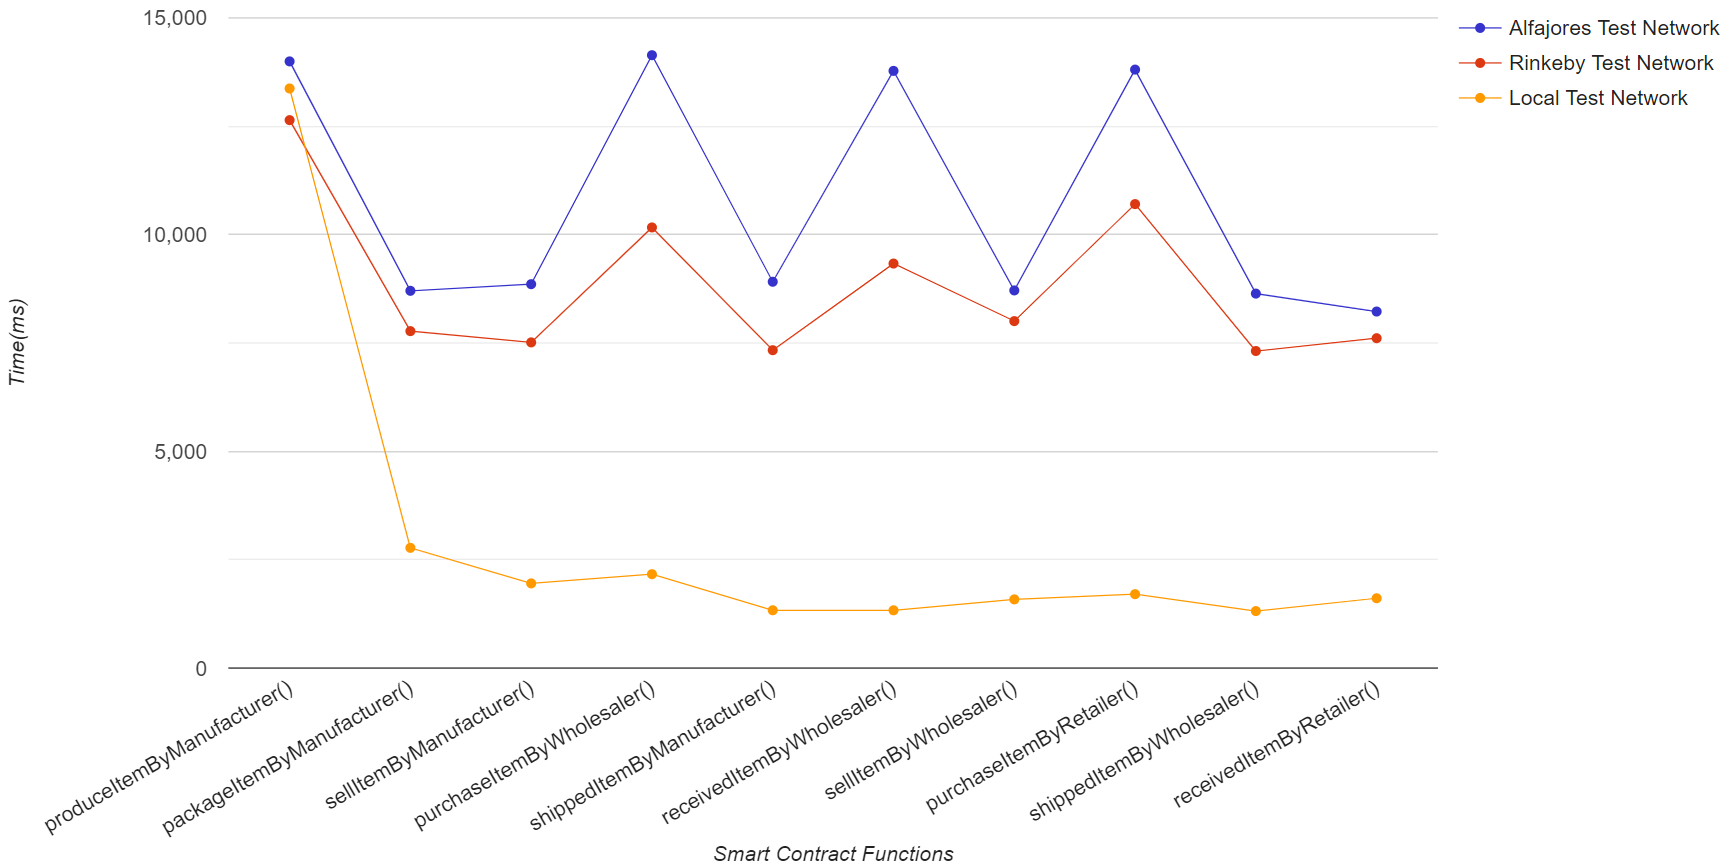
\includegraphics[width=15cm]{includes/figures/graph.png} 
  \caption{Performance across various networks}
  \label{Testing on networks}
\end{figure}

\vspace{.5cm}

It is obvious that the local network used far less time than the other two networks from figure \ref{Testing on networks}. However, it was simpler to obtain CELO for Alfajores, the blockchain currency we used as gas for deployment and payment, than it was to acquire RinkebyETH for the Rinkeby test network. On the other hand, we can see that contract deployment was a little faster using the Rinkeby test network compared to the Alfajores test network.


\begin{figure}[h]
\centering
  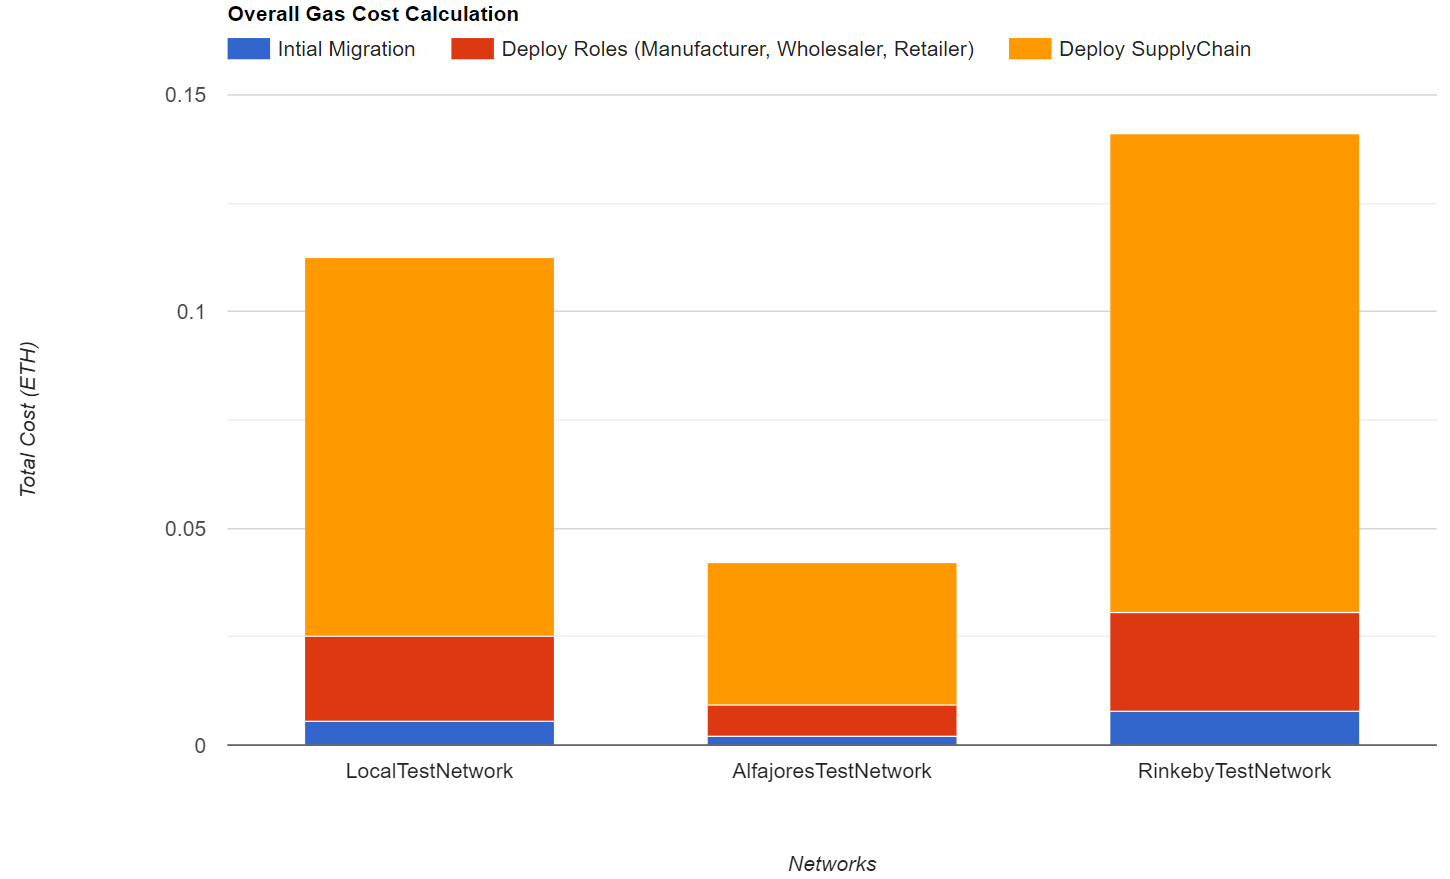
\includegraphics[width=11cm]{includes/figures/totalCost.png} 
  \caption{Overall deployment gas cost calculation }
  \label{Overall Gas Cost calculation}
\end{figure}

\vspace{.5cm}

The entire amount of gas utilized on a public testnet, such as alfajores and rinkeby, will depend on the network's present condition and resource demand. Due to the greater volume of transactions and contracts being executed on the public testnet, the overall gas consumption can be higher than on a local test network. In light of the fact that gas prices change on the public testnet as well, the total amount of gas utilized will also rely on those prices at the time of deployment and transaction. In figure \ref{Overall Gas Cost calculation}, The most expensive test network is rinkeby, however even though its gas consumption was same as alfajores test network's, alfajores' overall cost decreased to approximately one-third of rinkeby test network's cost due to low gas prices which was just 7.5 Gwei or 7500000000 Wei compared to rinkeby test network's gas price which was 20 Gwei or 20000000000 Wei.

\begin{figure}[h]
\centering
  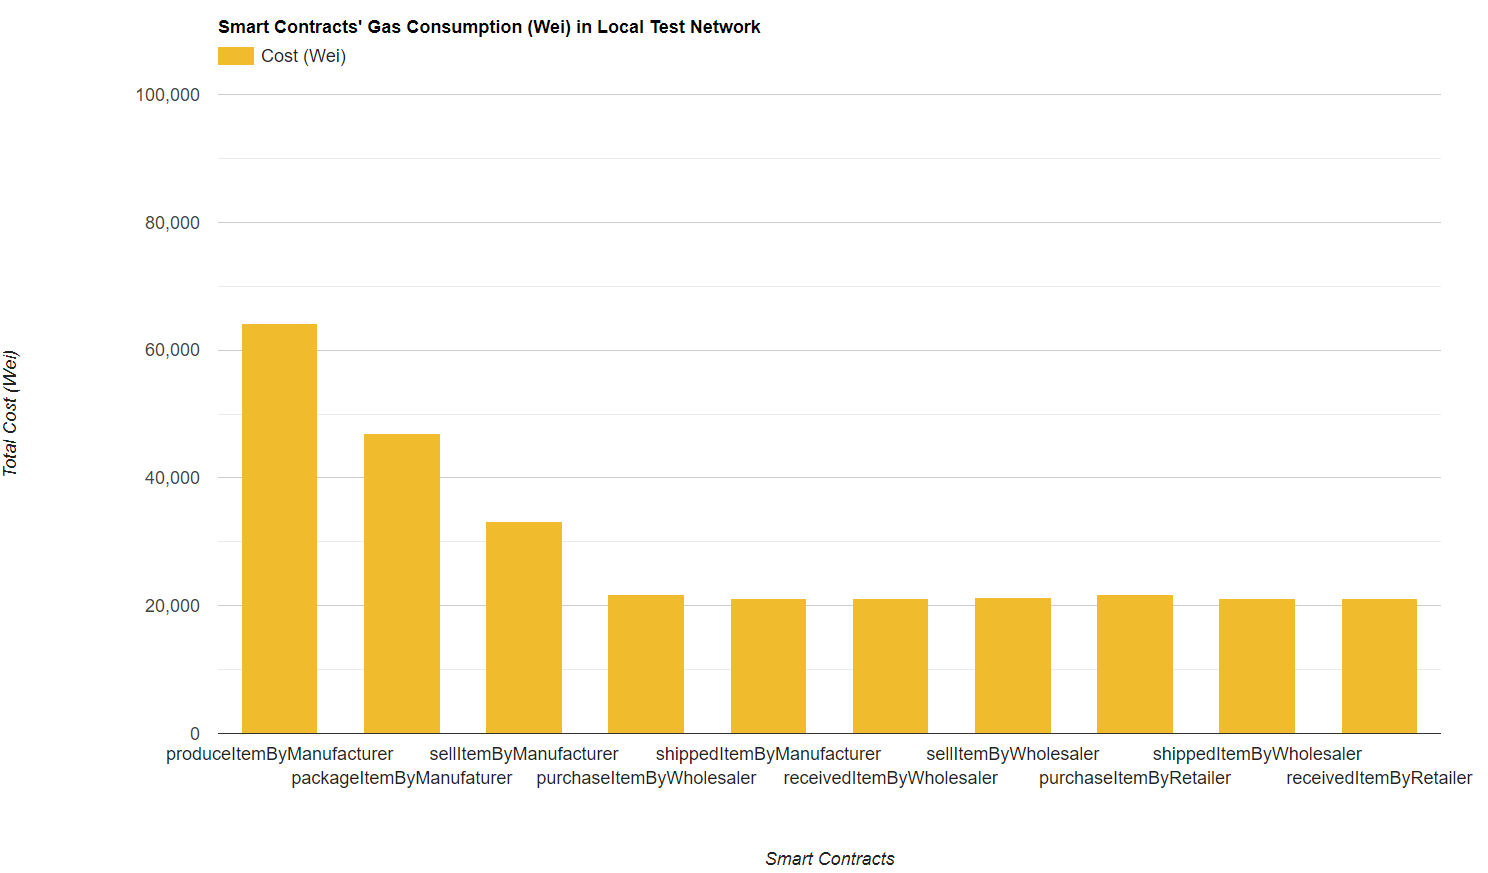
\includegraphics[width=12cm]{includes/figures/smartcontractgas.png} 
  \caption{Gas consumed by each smart contract}
  \label{Gas consumed by each contract}
\end{figure}

\vspace{.5cm}
The intricacy of the code, the volume of data being processed, and the present status of the network are some of the variables that affect how much gas will be required overall for a transaction or the deployment of a smart contract on a blockchain network. Because a local test network is less busy and has fewer resource demands than a public testnet like alfajores or rinkeby, the overall amount of gas utilized there is probably lower. Therefore, we selected the local test network to determine how much gas was used to generate each of the smart contracts as shown in figure \ref{Gas consumed by each contract}. We determined that the overall quantity of gas utilized might still vary depending on how much data is handled and how complicated the code is.


\subsubsection{Contract Language Analogy}

We were decided from the outset to utilize Solidity to construct the smart contracts since it is a curly-bracket language meant to target the \ac{EVM}. C++, Python, and JavaScript have all had an impact on it. Solidity is statically typed and, among other things, enables inheritance, libraries, and sophisticated user-defined types. Furthermore, it receives frequent upgrades and breaking modifications, and new features are released on a regular basis. 

\vspace{.5cm}

Jason's and some issue with web3 libraries gave us the opportunity to explore more and to switch from Solidity to Vyper and learn more about the language. Because Vyper lacks \textit{Modifiers}, \textit{Class Inheritance}, \textit{Inline Assembly}, \textit{Function Overloading}, \textit{Operator Overloading}, and \textit{Binary Fixed Point}, a thorough examination of Vyper prompted us to chose Solidity once more. The usage of the following constructs might result in confusing or challenging to comprehend code, hence they are not included and to create final smart contracts, we continued to use Solidity as our primary language.


\section{Infuse Blockchain Technology in Multiple Agent System}

Following the creation of contracts, we began looking for an appropriate \ac{AOP} language that is compatible with the \texttt{web3} library and can be used by agents in a \ac{MAS} to generate smart contracts. In the last chapter, we discussed every solution we considered. 

\subsubsection{Finale Outcome}

Our main objective was to find a way to incorporate \ac{BCT} into \ac{MAS} and create smart contracts using Jason \ac{BDI} agents. One of our ideas was successful, and the infuse was effective. We tested the code several times to make sure it was running correctly by looking at the \texttt{contract address} and \texttt{transaction hashes} from ganache as we were deploying using local network, and each try was successful, as can be seen in the output from one of the evaluations below.

\vspace{.5cm}

Also, regarding the quantity of stock in the warehouse and the batch order for the product, there are several scenarios that might occur. The results of each scenario are displayed below:

\vspace{.5cm}

\begin{itemize}
    \item Retailer's warehouse has sufficient product, so \texttt{RetailerAgent} doesn't need to order from \texttt{WholesalerAgent}.

    \vspace{.5cm}
    \begin{lstlisting}[numbers=none, basicstyle=\ttfamily\tiny]
    
    <---------------------SMART CONTRACTS AND AGENTS----------------------->
    Deployed Contract Address: 0xc9f78D73aCAf603Fe2319682316268A39Cc5CBB7
    Owner Address: accounts[0] 0xad0BC114B5CF3F0797346fF1Fb1Daf1Cf5123395
    Manufacturer Address: accounts[1] 0x4A9fe326Edc88F1f22940DC9F70BD391fB4218f8
    Wholesaler Address: accounts[2] 0x5fB0Cd136C7A19E8E12F062548002B4460B0dC0d
    Retailer Address: accounts[3] 0xc7D1C50D87B82E85b959DBC2cD9959bfc0480A5E
    <------------------------------------------------------------------------>
    
    <---------------------INTERACTION BETWEEN AGENTS-------------------->
    mainAgent           : Starting SupplyChain with SmartContracts
    mainAgent           : Hi, I am the owner of Contract, with account: 0xad0BC114B5CF3F0797346fF1Fb1Daf1Cf5123395
    mainAgent           : Creating RetailerAgent
    retailerAgent       : Hi, I am here, with account: 0xc7D1C50D87B82E85b959DBC2cD9959bfc0480A5E
    retailerAgent       : Checking Warehouse, and no need to order
    retailerAgent       : Giving products to supplyChainAgent
    mainAgent           : Selling to customers
    mainAgent           : SUPPLYCHAIN COMPLETE
    \end{lstlisting}
    
    \vspace{.5cm}
    
    \item Retailer's warehouse has insufficient product, so \texttt{RetailerAgent} need to order from \texttt{WholesalerAgent} and Wholesaler's warehouse has sufficient product, so \texttt{WholesalerAgent} doesn't need to order from \texttt{ManufactureAgent}.

    \vspace{.5cm}
    \begin{lstlisting}[numbers=none, basicstyle=\ttfamily\tiny]
    <---------------------SMART CONTRACTS AND AGENTS----------------------->
    Deployed Contract Address: 0xc9f78D73aCAf603Fe2319682316268A39Cc5CBB7
    Owner Address: accounts[0] 0xad0BC114B5CF3F0797346fF1Fb1Daf1Cf5123395
    Manufacturer Address: accounts[1] 0x4A9fe326Edc88F1f22940DC9F70BD391fB4218f8
    Wholesaler Address: accounts[2] 0x5fB0Cd136C7A19E8E12F062548002B4460B0dC0d
    Retailer Address: accounts[3] 0xc7D1C50D87B82E85b959DBC2cD9959bfc0480A5E
    <------------------------------------------------------------------------>
    
    <---------------------INTERACTION BETWEEN AGENTS-------------------->
    mainAgent           : Starting SupplyChain with SmartContracts
    mainAgent           : Hi, I am the owner of Contract, with account: 0xad0BC114B5CF3F0797346fF1Fb1Daf1Cf5123395
    mainAgent           : Creating RetailerAgent
    retailerAgent       : Hi, I am here, with account: 0xc7D1C50D87B82E85b959DBC2cD9959bfc0480A5E
    retailerAgent       : Checking Warehouse
    retailerAgent       : INSUFFICIENT INVENTORY!! Ordering Product..
    retailerAgent       : Ordering to wholesalerAgent
    mainAgent           : Creating WholesalerAgent
    wholesalerAgent     : Hi, I am here, with account: 0x5fB0Cd136C7A19E8E12F062548002B4460B0dC0d
    wholesalerAgent     : Checking Warehouse, and no need to order
    wholesalerAgent     : Selling product to retailerAgent
    wholesalerAgent     : Tx sellItemByWholesaler successful with hash: 0x421c5ed80a71376a4e8e4e7b6a4083bd8e83f734ed43c67130847eab0f2c7fdf
    retailerAgent       : Purchasing product from wholesalerAgent
    retailerAgent       : Tx purchaseItemByRetailer successful with hash: 0xc07aba5f53bb5d74ce1aea3d788d0c65cb34a036a1459750e9d2db6d9e81cda0
    wholesalerAgent     : Shipping product to retailerAgent
    wholesalerAgent     : Tx shippedItemByWholesaler successful with hash: 0x33e0b25c8d44b837b573ed00e1fe34315c6de613fcacfa2856a4f1cb10671be3
    retailerAgent       : Received product from wholesalerAgent and Inventory full!!
    retailerAgent       : Tx receivedItemByRetailer successful with hash: 0xcc84c9fe3cd74b803419e4dde53f71f0d01243ea0d4ec1873b5aadb95cba23e2
    retailerAgent       : Checking Warehouse, and no need to order
    retailerAgent       : Giving products to supplyChainAgent
    mainAgent           : Selling to customers
    mainAgent           : SUPPLYCHAIN COMPLETE
    \end{lstlisting}
    
    \vspace{.5cm}

    \item Retailer's warehouse has insufficient product, so \texttt{RetailerAgent} need to order from \texttt{WholesalerAgent}, Wholesaler's warehouse has also insufficient product, so \texttt{WholesalerAgent} need to order from \texttt{ManufactureAgent} and Manufacture's warehouse has sufficient product, so \texttt{ManufactureAgent} doesn't need to manufacture product.

    \vspace{.5cm}
    \begin{lstlisting}[numbers=none, basicstyle=\ttfamily\tiny]
    <---------------------SMART CONTRACTS AND AGENTS----------------------->
    Deployed Contract Address: 0xc9f78D73aCAf603Fe2319682316268A39Cc5CBB7
    Owner Address: accounts[0] 0xad0BC114B5CF3F0797346fF1Fb1Daf1Cf5123395
    Manufacturer Address: accounts[1] 0x4A9fe326Edc88F1f22940DC9F70BD391fB4218f8
    Wholesaler Address: accounts[2] 0x5fB0Cd136C7A19E8E12F062548002B4460B0dC0d
    Retailer Address: accounts[3] 0xc7D1C50D87B82E85b959DBC2cD9959bfc0480A5E
    <------------------------------------------------------------------------>
    
    <---------------------INTERACTION BETWEEN AGENTS-------------------->
    mainAgent            : Starting SupplyChain with SmartContracts
    mainAgent            : Hi, I am the owner of Contract, with account: 0xad0BC114B5CF3F0797346fF1Fb1Daf1Cf5123395
    mainAgent            : Creating RetailerAgent
    retailerAgent        : Hi, I am here, with account: 0xc7D1C50D87B82E85b959DBC2cD9959bfc0480A5E
    retailerAgent        : Checking Warehouse
    retailerAgent        : INSUFFICIENT INVENTORY!! Ordering Product..
    retailerAgent        : Ordering to wholesalerAgent
    mainAgent            : Creating WholesalerAgent
    wholesalerAgent      : Hi, I am here, with account: 0x5fB0Cd136C7A19E8E12F062548002B4460B0dC0d
    wholesalerAgent      : Checking Warehouse
    wholesalerAgent      : INSUFFICIENT INVENTORY!! Ordering Product..
    wholesalerAgent      : Ordering to manufacturerAgent
    mainAgent            : Creating ManufacturerAgent
    manufacturerAgent    : Hi, I am here, with account: 0x4A9fe326Edc88F1f22940DC9F70BD391fB4218f8
    manufacturerAgent    : Checking Warehouse
    manufacturerAgent    : Quantity alread exist in inventory, dont need to manufacture!
    manufacturerAgent    : Selling product to wholesalerAgent
    manufacturerAgent    : Tx sellItemByManufacturer successful with hash: 0x95c053089529888fb8c399355e666e6827935cc1b3e45b4bce90ccbc07eccd6b
    wholesalerAgent      : Purchasing product from manufacturerAgent
    wholesalerAgent      : Tx purchaseItemByWholesaler successful with hash: 0x28719d94c2f40383a74c25d39859dc4a1f26b06d0adb6d39f5e20ab7a5f6f499
    manufacturerAgent    : Shipping product to wholesalerAgent
    manufacturerAgent    : Tx shippedItemByManufacturer successful with hash: 0x5cbf427497b18c441dc7d44808cfd522c1f62e41a0c7c8524acb63a8aa8b4461
    wholesalerAgent      : Received product from manufacturerAgent, and added to the inventory and Inventory FULL!!
    wholesalerAgent      : Tx receivedItemByWholesaler successful with hash: 0x3ff03e21cd1b42eea4a55504dca701cd16484408acd9831f7f6a5df216f46e2e
    wholesalerAgent      : Checking Warehouse, and no need to order
    wholesalerAgent      : Selling product to retailerAgent
    wholesalerAgent      : Tx sellItemByWholesaler successful with hash: 0x5a786f97f9ff516c319e1473c8fff3b850c68010ea37ea32778f8f53e6704090
    retailerAgent        : Purchasing product from wholesalerAgent
    retailerAgent        : Tx purchaseItemByRetailer successful with hash: 0xb2a75b53a5f4ee86551a6a31d8324fd807376c2bc03a0a6b3d0585f5819be626
    wholesalerAgent      : Shipping product to retailerAgent
    wholesalerAgent      : Tx shippedItemByWholesaler successful with hash: 0x3fc8c3f81c033257ab58c5f9ca09197e7eafe7a61a6df4ba9b60e054ed7fb42a
    retailerAgent        : Received product from wholesalerAgent
    retailerAgent        : Tx receivedItemByRetailer successful with hash: 0x70660ae51b082f39a551e8c0132058c1bbc557267826ecd81ed59006025b5722
    retailerAgent        : Checking Warehouse, and no need to order
    retailerAgent        : Giving products to supplyChainAgent
    mainAgent            : Selling to customers
    mainAgent            : SUPPLYCHAIN COMPLETE
    \end{lstlisting}
    
    \vspace{.5cm}

    \item Retailer's warehouse has insufficient product, so \texttt{RetailerAgent} need to order from \texttt{WholesalerAgent}, Wholesaler's warehouse has also insufficient product, so \texttt{WholesalerAgent} need to order from \texttt{ManufactureAgent} and Manufacture's warehouse has also insufficient product, so \texttt{ManufactureAgent} needs to manufacture product. In this scenario, \texttt{WholesalerAgent} ordered again because it wanted to make its inventory full. 

    \vspace{.5cm}
    \begin{lstlisting}[numbers=none, basicstyle=\ttfamily\tiny]
    <---------------------SMART CONTRACTS AND AGENTS----------------------->
    Deployed Contract Address: 0xc9f78D73aCAf603Fe2319682316268A39Cc5CBB7
    Owner Address: accounts[0] 0xad0BC114B5CF3F0797346fF1Fb1Daf1Cf5123395
    Manufacturer Address: accounts[1] 0x4A9fe326Edc88F1f22940DC9F70BD391fB4218f8
    Wholesaler Address: accounts[2] 0x5fB0Cd136C7A19E8E12F062548002B4460B0dC0d
    Retailer Address: accounts[3] 0xc7D1C50D87B82E85b959DBC2cD9959bfc0480A5E
    <------------------------------------------------------------------------>
    
    <---------------------INTERACTION BETWEEN AGENTS-------------------->
    mainAgent            : Starting SupplyChain with SmartContracts
    mainAgent            : Hi, I am the owner of Contract, with account: 0xad0BC114B5CF3F0797346fF1Fb1Daf1Cf5123395
    mainAgent            : Creating RetailerAgent
    retailerAgent        : Hi, I am here, with account: 0xc7D1C50D87B82E85b959DBC2cD9959bfc0480A5E
    retailerAgent        : Checking Warehouse
    retailerAgent        : INSUFFICIENT INVENTORY!! Ordering Product..
    retailerAgent        : Ordering to wholesalerAgent
    mainAgent            : Creating WholesalerAgent
    wholesalerAgent      : Hi, I am here, with account: 0x5fB0Cd136C7A19E8E12F062548002B4460B0dC0d
    wholesalerAgent      : Checking Warehouse
    wholesalerAgent      : INSUFFICIENT INVENTORY!! Ordering Product..
    wholesalerAgent      : Ordering to manufacturerAgent
    mainAgent            : Creating ManufacturerAgent
    manufacturerAgent    : Hi, I am here, with account: 0x4A9fe326Edc88F1f22940DC9F70BD391fB4218f8
    manufacturerAgent    : Checking Warehouse
    manufacturerAgent    : INSUFFICIENT INVENTORY!! Manufacturing Product..
    manufacturerAgent    : Tx produceItemByManufacturer successful with hash: 0xde3468f453048739395cfe770a2be70654ac05d7fe006fd77ad2e91e55cd0fb5
    manufacturerAgent    : Packaging Product
    manufacturerAgent    : Tx packageItemByManufacturer successful with hash: 0xac339f4c9d1bd18c206c4fefa2da1578255ab184cfb56a19aa5f0c749691c90f
    manufacturerAgent    : Checking Warehouse
    manufacturerAgent    : Quantity alread exist in inventory, dont need to manufacture!
    manufacturerAgent    : Selling product to wholesalerAgent
    manufacturerAgent    : Tx sellItemByManufacturer successful with hash: 0x70d3e37c5cae73f9e3721dd1cec079b2329f241d035bc3c0d8d5435c9980291a
    wholesalerAgent      : Purchasing product from manufacturerAgent
    wholesalerAgent      : Tx purchaseItemByWholesaler successful with hash: 0x45057874c25a62ad149fc3e984a6856fc8ca3865fe8f1faa558e237b84437a87
    manufacturerAgent    : Shipping product to wholesalerAgent
    manufacturerAgent    : Tx shippedItemByManufacturer successful with hash: 0x9ae2c0454a62266658d252827a852d8c4f2636ce106e5fe122c0a0fce1f49518
    wholesalerAgent      : Received product from manufacturerAgent, and added to the inventory and and Inventory not full yet!!
    wholesalerAgent      : Tx receivedItemByWholesaler successful with hash: 0x7b2b32121504e0c424faf0721aba7dde1152781d8e6ca099146bca2a99321863
    manufacturerAgent    : Selling product to wholesalerAgent Again
    manufacturerAgent    : Tx sellItemByManufacturer successful with hash: 0xb5b7ed54756b9123522d942c131f52a79450ed8a61b5b5f17b5e762c4dfd2c96
    wholesalerAgent      : Purchasing product from manufacturerAgent Again
    wholesalerAgent      : Tx purchaseItemByWholesaler successful with hash: 0x0000ce3707589a17982b27b0efb13872ffc8b2c8ff509e3783f19fa2e81a2263
    manufacturerAgent    : Shipping product to wholesalerAgent
    manufacturerAgent    : Tx shippedItemByManufacturer successful with hash: 0xdc4e1db2675c4a85b20eca1ce2e94ce9064ae8ec4d7160c23f5dc3e682e714b1
    wholesalerAgent      : Received product from manufacturerAgent, and added to the inventory and Inventory FULL!!
    wholesalerAgent      : Tx receivedItemByWholesaler successful with hash: 0x130f6ac86210088f05687b9d769615856bc0da2459c5ff68640330c2e8ffcf66
    wholesalerAgent      : Tx receivedItemByWholesaler successful with hash: 0xe37eb45b7918a377f96daaf95be30432d2c8902f3033c0809fc3a1ec0970bcf5
    wholesalerAgent      : Checking Warehouse, and no need to order
    wholesalerAgent      : Selling product to retailerAgent
    wholesalerAgent      : Tx sellItemByWholesaler successful with hash: 0x6aaf996c1a2347612b38350cc31c20320d25d21da80878be1776cbd1f8138258
    retailerAgent        : Purchasing product from wholesalerAgent
    retailerAgent        : Tx purchaseItemByRetailer successful with hash: 0x18677b7134c6ee338ac749c090e4121f2fa80308837da9f1c8f13955841e411a
    wholesalerAgent      : Shipping product to retailerAgent
    wholesalerAgent      : Tx shippedItemByWholesaler successful with hash: 0x45e406258e946a2eee2969dbf5461c799d036190598677a3b787b3e93bbf9ddd
    retailerAgent        : Received product from wholesalerAgent
    retailerAgent        : Tx receivedItemByRetailer successful with hash: 0x24d53dcdb1b44e2b86938daa9df29ad8efd7f40718a73d0f3a4aff9437c2f68f
    retailerAgent        : Checking Warehouse, and no need to order
    retailerAgent        : Giving products to supplyChainAgent
    mainAgent            : Selling to customers
    mainAgent            : SUPPLYCHAIN COMPLETE
    \end{lstlisting}
    
    \end{itemize}


The output above demonstrates how the various supply chain roles interact with one another to complete the process of planning, manufacturing, and delivering a product or service. It demonstrates that each role has been given an \texttt{account number} and that whenever they interact or complete a procedure, a \texttt{transaction hash} is issued to verify its authenticity and for future use.

\vspace{.5cm}

After a successful implementation, we remained adamant about running it in Java and used the \texttt{web3j} package to integrate \ac{BCT} into \ac{MAS}. We attempted to use Jason with Java by converting the Python code into a Java application. The creation of a Java application containing Python code was successful, but when the \texttt{.mas2j} file was executed, but it was unable to import the package \texttt{org.python}, which is necessary to start the program.